\documentclass[12pt]{article}
\usepackage{amsmath}
\usepackage{amssymb}
\usepackage{graphicx}
\usepackage{comment}
\usepackage{longtable}
\usepackage{graphicx}

\begin{document}

\title{\textbf{REQUIREMENTS ANALYSIS DOCUMENT }}
\maketitle

\begin{center}
\title{\textbf{Software Design COMS3009}}
\maketitle
\end{center}
\begin{center}
\title{\textbf{FindMeTutor Android Application}}
\maketitle
\end{center}

\begin{center}
Proposed idea by:\\
Shaneel James-718840
\\Jadon Manilal-815050
\\Jared Naidoo - 719238
\\Krupa Prag - 782681
\\Nivek Ranjith - 802119
\end{center}


\newpage
%TABLE OF CONTENTS
\tableofcontents
\newpage


\section{\textbf{Executive Summary}}
\begin{flushleft}
The problem that we face is that students are in need of extra lessons and tutorials outside of standard lessons provided by the university. We propose a system that can connect students in search of tutors.

The results of the requirements analysis are documented below. This document completely describes the system in terms of the requirements. This document serves as a contextual basis between the client and the developer.
\end{flushleft}
\newpage
%INTRODUCTION
\section{INTRODUCTION}
\subsubsection{Purpose of the system}
\begin{flushleft}
The purpose of the FindMeTutor application is to provide a convenient means for tutors and students who are looking for tutors to be able to connect within a particular tertiary institute.
\end{flushleft}
\subsubsection{Scope of the system}
\begin{flushleft}
Our team, working on the FindMeTutor application, envisions a successful product to be an Android Application which will be at a students disposal in order to improve their grades and achieve their academic dreams. With limited resources, a stringent budget and capped time, we aim to execute this task in an economical fashion.\\
This goal will be achieved by making use of agile methodology. We will be able to set short term targets to achieve deliverables within sprints, with a long term goal being to present the FindMeTutor Android Application.
\end{flushleft}
\subsubsection{Objective and success criteria of the project}
\begin{flushleft}
The FindMeTutor Android application will be seen as successful if it facilitates a platform on which tutors and students can meet. We have great hope that the result of this would mean better results obtained by the students, and a manner in which tutors can generate some income and gain some job experience.
\end{flushleft}
\subsubsection{Definitions, acronyms, and abbreviations}
1. App - abbreviation for application. \\
2. Application - is a piece of software \\
3. Android - is a mobile operating system developed by Google. \\
4. OS - abbreviation for operating system.\\
5. Operating system - is a collection of software that communicates with hardware and allows other programs to run on it.\\
6. Java - is a high-level programming language\\
7. UI - abbreviation for User interface\\
8. User interface/GUI - is the means in which a person controls a software application or hardware device.\\
9. ID - abbreviation for identity\\
11.User ID - the idenity that uniquely identifies someone on a computer system.\\
12. Sign in - when asked to enter username and password information. A sign in/login is a combination of information that authenticates a user's identity. \\
13. SDK - abbreviation for Software Development Kit\\
14 Software Development Kit -  collection of software used for developing applications for a specific device or operating system.
15 Sessions - A tutorial session created by a student.

\subsubsection{References}
1. http://techterms.com/definition (2016-08-08)
%\subsubsection{Overview}
%dummy text
\newpage

%CURRENT SYSTEM
\section{CURRENT SYSTEM}
\subsubsection{Overview}
\begin{flushleft}
Currently, there are many students in search of tutors to help them with particular courses with which they require some support, as well as fellow students or tutors who are available to tutor particular courses of study. However, the problem that is faced on hand is that either pool (students and tutors) are struggling to find each other.
\end{flushleft}

\newpage

%PROPOSED SYSTEM
\section{PROPOSED SYSTEM}
\subsection{Overview}
\begin{flushleft}
FindMeTutor app will be a platform through which students and tutors can meet in order to resolve the current situation.
\end{flushleft}
\begin{flushleft}
FindMeTutor app will facilitate the following two registration categories:

\begin{flushleft}
1.Student looking for tutors – they are able to register on the app with merely some personal details (demographic data, email and password).\\
2. Tutor - those who would like to tutor can register on the app by simply filling in some details with respect to the fields of study they are particularly comfortable to tutor.\\
\end{flushleft}
\end{flushleft}
\subsection{Functional requirements - "Shall lists"}

Describes the high-level functionality of the system\\

\begin{comment}
3.2.1 The database has the ability to store data captured of the users of the application (student and tutors data).More specifically, the database will be able to accept numeric data entry and will store the courses under the University of the Witwatersrand's School of Computer science and Applied mathematics undergraduate topics which will be displayed in the drop-down menu when students and tutors will be required to select the courses respectively to which they are enrolled in or able to tutor. \\
3.2.2 The app will provide an effective means through which tutors and students can communicate. The messenger facility will facilitate communication between students and tutors - when students request a tutor, the tutor and student will be able to use this facility to arrange a convenient time, place and tuition fee for the tutor service. \\
3.2.3 Request appropriate tutors for students who send a request on the app for a tutor eligible to tutor a specific course (aid to pair up appropriate tutors and students).\\
3.2.4 In the light of security, the database shall be able store a corresponding password for each user of the application, which will allow for each users account to be protected, as each user's users email address and entered password will be compared to that of which was entered into the database at sign-up, hence the system restricting access to authorized users. \\
3.2.5 FindMeTutor Android application will be able to be utilised on any Android OS of (some version), which is able easily accessible,as many students can download this application for use on their smartphones and/or tablets which shall makes the application easily accessible.
\end{comment}

\begin{flushleft}
\textbf{Overview of Requirements}
\end{flushleft}
{
\centering
\begin{longtable}{| p{1.5cm} | p{13.5cm}|  }
\hline
\textbf{Item} & \textbf{Requirements to implement}

% Proposal
	\\ \hline 0 & Proposal
% Student Registration
		\\ \hline 1 & Student registration and login \\ \hline

%Tutor Registration
			2 & Tutor registration and login \\ \hline

% System Administrator Registration
			3 & Administrator registration  \\ \hline


% Administrator capabilities
			4 & Administrator capabilities\\ \hline

% Request tutor: student
			5 & Students able to request a tutor\\ \hline

% Request Tutor: Tutor
				6 & Tutor able to accept/reject tutor requests\\ \hline

% Add Event: Student
				7 & Student able to handle 'Upcoming events'   \\ \hline

% Add Event: Tutor
				8 & Tutor able to handle 'Upcoming events'  \\ \hline

% Rate a tutor: student
				9 & Student able to rate a tutor \\ \hline

% Check-in/out : Sudent
				10 & Student able to check-in/check-out of tutor sessions  \\ \hline

% Safety checker
				11 & Tutors able to check-in/check-out of tutor sessions   \\ \hline

% Payment
				12 & Student funding and payment \\ \hline
% Payment
				13 & Tutor funding and payment \\ \hline
% subjects
				14 & Students able to add/ remove subjects enrolled in\\ \hline
% subjects
				15 & Tutors able to add/ remove subjects able to tutor\\ \hline
% Login
				16 & Login of student and tutors\\ \hline
% Sessions
				17 & Students and tutors can log their tutorial sessions\\ \hline
% Archive account
				18 & Students and tutors can mark off completed sessions\\ \hline


\end{longtable}
}


{
\centering
\begin{longtable}{| l | p{10cm}| l |}
			\hline
			\textbf{Requirement} & \textbf{Functional Requirement} & \textbf{Use Case}

			\\ \hline RQ1.1 & The system shall allow a student to register  & UC-CS \\ \hline
			RQ1.2 & The system shall allow a student to update their account eg update password& UC-US \\ \hline
			RQ1.3 & The system shall allow a student to view their account details  & UC-VS \\ \hline
			RQ1.4 & The system shall allow a student to mark their account as deleted & UC-DS  \\ \hline

			RQ2.1 & The system shall allow a tutor to register & UC-CT \\ \hline
			RQ2.2 & The system shall allow a tutor to update their account eg password update & UC-UT \\ \hline
			RQ2.3 & The system shall allow a tutor to view their account details & UC-VT \\ \hline
			RQ2.4 & The system shall allow a tutor to mark their account as deleted & UC-DT \\ \hline

		%	RQ3.1 & The system shall allow an administrator to update a student account & UC-US \\ \hline
		%	RQ3.2 & The system shall allow an administrator to view a student account details  & UC-VS \\ \hline
		%	RQ3.3 & The system shall allow an administrator to mark a student as deleted & UC-DS  \\ \hline
		%	RQ3.4 & The system shall allow an administrator to update a tutor account eg update password & UC-UT \\ \hline
		%	RQ3.1 & The system shall allow an administrator to view a tutor account details & UC-VT \\ \hline
		%	RQ3.2 & The system shall allow an administrator to mark a tutor account as deleted & UC-DT \\ \hline

% Ask if we have the password under update

% Create Administrator
		%	RQ4.1 & The system shall allow an administrator to register  & UC-CA \\ \hline
		%	RQ4.2 & The system shall allow an administrator to update their account & UC-UA \\ \hline
		%	RQ4.3 & The system shall allow an administrator to view their account details  & UC-VA \\ \hline
		%	RQ4.4 & The system shall allow an administrator to mark their account as deleted & UC-DA  \\ \hline

% Request tutor: student
				RQ3.1 & The system shall allow a student to request a tutor & UC-RT \\ \hline
				RQ3.2 & The system shall allow a student to choose a tutor from a list & UC-RT \\ \hline

% Request Tutor: Tutor
				RQ4.1 & The system shall allow a tutor to accept a request & UC-RT \\ \hline
				RQ4.2 & The system shall allow a tutor to reject a request & UC-RT \\ \hline




% Rate a tutor: student
				RQ5.1 & The system shall allow a student to rate a tutor & UC-R\\ \hline

% Check-in/out : Sudent
				RQ6.1 & The system shall allow a student to check-in  & UC-CI \\ \hline
				RQ6.2 & The system shall allow a student to check-out  & UC-CO \\ \hline
% Check-in/out : Tutor
				RQ7.1 & The system shall allow a tutor to check-in  & UC-CI \\
\hline
				RQ7.2 & The system shall allow a tutor to check-out  & UC-CO \\ \hline
				RQ8.1 & The system shall allow a student to add funds &UC-CF\\ \hline
				RQ8.2 & The system shall allow a student to view funds &UC-VF\\ \hline
				RQ8.3 & The system shall allow a student to update funds &UC-UF\\ \hline
				RQ9.1 & The system shall allow a tutor to add funds &UC-CF\\ \hline
				RQ9.2 & The system shall allow a tutor to view funds &UC-VF\\ \hline
				RQ9.3 & The system shall allow a tutor to update funds &UC-UF\\ \hline
				RQ10.1 & The system shall allow a student to add subjects &UC-CSb\\ \hline
				RQ11.1 & The system shall allow a tutor to add subjects &UC-CSb\\ \hline
				RQ12.1 & The system shall allow a student to remove subjects &UC-DSb\\ \hline
				RQ12.2 & The system shall allow a tutor to remove subjects &UC-DSb\\ \hline
				RQ13.1 & The system shall allow a student to login &UC-L\\ \hline
				RQ13.2 & The system shall allow a tutor to login &UC-L\\ \hline
				%RQ16.3 & The system shall allow an administrator to login &UC-L\\ \hline
				RQ14.1 & The system shall allow a student to view their upcoming sessions  &UC-VSes\\ \hline
				RQ14.2 & The system shall allow a tutor to view their upcoming sessions  &UC-VSes\\ \hline
				RQ15.1 & The system shall allow a tutor to mark a session as done &UC-DSes\\ \hline
				RQ15.2 & The system shall allow a student to mark a session as done &UC-DSes\\ \hline
				RQ16.1 & The system shall allow a tutor to mark a session as cancelled &UC-DSes\\ \hline
				RQ16.2 & The system shall allow a student to mark a session as cancelled &UC-DSes\\ \hline
				RQ17.1 & The system shall allow a student to view a subject &UC-RSb\\ \hline
				RQ17.2 & The system shall allow a tutor to view a subject &UC-RSb\\ \hline
				%Sprint3
				RQ18.1 & The system shall allow a students account to automatically be deducted from their account to make a payment to the tutor, once they both have checked out  &UC-FP\\ \hline
				RQ18.2 & The system shall allow a tutor receive funds from a student once they both check-out of a tutorial session &UC-FP\\ \hline
\end{longtable}
}
\subsection{Functional requirements specification}
%Although this section is entitled “Requirements Specification,” we will see that we
%are still discovering the functional system requirements for the system-to-be, as
%well as specifying the discovered requirements.
\subsubsection{Stakeholders}
%Identify anyone and everyone who has interest in this system (users, managers, sponsors, etc.).
%Stakeholders should be humans or human organizations.
\begin{itemize}
\item Students
\item Tutors
\item University (Facculty of Science : School of Computer Science and Applied Mathematics)
\end{itemize}
\subsubsection{Actors and Goals}
\begin{itemize}
\item Students - a registered user looking for a tutor
\item Tutors - a registered user, whom is approachable to tutor particular subjects
\item Database - records details of students and tutors. Stores required information with regards to tutorials for student and tutor.
\end{itemize}

\subsection{Non-functional requirements}{
Describes the user-level requirements that are not directly related to the functionality. \\
\\\textbf{3.3.1 Usability}\\
The application will be user friendly as it will be an Android application which is supported by multiple devices (android smartphones and android tablets). This will allow for the application to be easily accessible to students and tutors as majority of students have access to android devices.
\\\textbf{3.3.2 Reliability}\\
The probability that the system will be able to process work correctly and completely without being aborted.\\
In the case of system failure, the damage that could be caused could be such where a user will not be able to use the app during system failure.
\\\textbf{3.3.3 Performance}\\
%The expected volume of data (??).
The response time between the UI and the server will be optimised. The expected volume of user activity will peak at the end of each academic term within the tertiary institute when examinations/tests will be approaching, while on a regular basis the application will be utilised when students who feel the need to get assistance when they encounter a topic they require assistance in.
\\\textbf{3.3.4 Supportability}\\
The App will be facilitated over a spectrum of Android platform versions. The SDK supports 14-24. \\
\textbf{3.3.5 Implementation}\\
Our team has implemented the agile methodology in order to obtain our final goal of building the FindMeTutor application. For each sprint we will set targets of what we would like to achieve, with the objective of using these milestones to be building blocks towards our final goal.
\\\textbf{3.3.6 Interface}\\
The UI will be made in Android studio. The set up will be simple and neat. The app will be used by students who will be using the app in order to search for a tutor which is suitable to tutor, hence, with this intention, to prevent furthering the overwhelmed feeling, the app will not be clutered and simple to use. The 'user-friendly' experience provided by the UI, will allow the user to interact with the app in a natural and intuitive way. \\
Each user's home page will be customized to display there upcoming tutorial sessions.\\
\textbf{3.3.7 Packaging}\\
Android studio for development\\
Adobe illustrator and photoshop for App graphics - FindMeTutor logo\\
%\textbf{3.3.8 Legal}\\
}



\subsection{Acceptance Testing}
\subparagraph{Acceptance Test general}
\begin{itemize}
\item ACT0.01	Ensure working connection between the applcation and it's database (pass: database stores information and app displays required data from database)
%Student registration
\item ACT1.01	Challenge registered student to re-register with taken username (fail)
\item ACT1.02	Challenge new student to register with new identifier (pass)
\item ACT1.03	Challenge registered student to update their account (pass)
\item ACT1.04	Challenge registered student to view their account (pass)
%Tutor registration
\item ACT2.01	Challenge registered tutor to re-register with taken username (fail)
\item ACT2.02	Challenge new tutor to register (pass)
\item ACT2.03	Challenge registered tutor to update their account (pass)
\item ACT2.04	Challenge registered tutor to view their account (pass)
% Administrator capabilities
\item ACT3.01	Challenge registered administrator to view a registered student's account (pass)
\item ACT3.02	Challenge registered administrator to update a registered student's account (pass)
\item ACT3.03	Challenge registered administrator to mark a registered student's account as deleted (pass)
\item ACT3.04	Challenge registered administrator to view a registered tutor's account (pass)
\item ACT3.05	Challenge registered administrator to update a registered tutor's account (pass)
\item ACT3.06	Challenge registered administrator to mark a registered tutor's account as deleted (pass)
%Administrator registration
\item ACT4.01	Challenge registered administrator to re-register with taken username(fail)
\item ACT4.02	Challenge new administrator to register (pass)
\item ACT4.03	Challenge registered administrator to update their account (pass)
\item ACT4.04	Challenge registered administrator to view their account (pass)
% Request tutor: student
\item ACT5.01	A student requesting a tutor can request a tutor for a date/time which has already passed  (fail)
\item ACT5.02	A student requesting a tutor can request a tutor for a subject that they have not added to their enrolled subjects  (fail)
\item ACT5.03	A student requesting a tutor can request tutorials for various topics at a given time. ie. Student can request tutor for subject B while request tutor status for subject A is still pending (pass)
\item ACT5.04	A student requesting a tutor can delete a request for a  tutorial, if no longer require it. (fail)
\item ACT5.05	A student receiving a tutor acceptance notification, can agree to a tutorial session from the list  of tutors who have agreed (pass)
\item ACT5.06 A student receiving a tutor acceptance notification, can disagree to tutorial . ie . They can decide to no longer want to continue with the tutorial, or have selected another tutor who has accepted their request.(pass)		% Request tutor: tutor
\item ACT 6.01 A tutor can accept/reject a tutor request(pass)
% Add events: Students
\item ACT 7.01 A student can add an event to their upcoming events (pass)
\item ACT 7.02 A student can modify an event to their upcoming events (pass)
\item ACT 7.03 A student can delete an event to their upcoming events (pass)
\item ACT 7.04 A student can view an event to their upcoming events (pass)
% Add events: tutor
\item ACT 8.01 A tutor can add an event to their upcoming events (pass)
\item ACT 8.02 A tutor can modify an event to their upcoming events (pass)
\item ACT 8.03 A tutor can delete an event to their upcoming events (pass)
\item ACT 8.04 A tutor can view an event to their upcoming events (pass)
% Rate a tutor
\item ACT 9.01 A student can rate a tutor that they have previously had a tutorial session with. (pass)
\item ACT 9.02 A student can rate a tutor that they have not previously had a tutorial session with. (fail)
% Check-in
\item ACT 10.01 A student can check-in once at tutorial venue(pass)
% Check-in
\item ACT 11.01 A tutor can check-in once at tutorial venue(pass)
% funding and payment: Student
\item ACT 12.01 A student can pay in funds to their account balance (pass)
\item ACT 12.02 A student can view balance of their account funds (pass)
% funding and payment: Tutor
\item ACT 13.01 A tutor can receive funds toward their account baance - from student tutorial session payments (pass)
\item ACT 13.02 A tutor can view the balance of their account funds (pass)
% Add enrolled subjects: Students / Tutor
\item ACT 14.01 A student can add subjects in which they are enrolled(pass)
\item ACT 14.02 A tutor can add subjects in which they are fit to tutor(pass)
% remove subjects: students and  tutor
\item ACT 15.01 A student can remove subjects in which they are no longer enrolled(pass)
\item ACT 15.02 A tutor can remove subjects in which they no longer would want to tutor(pass)
% login
\item ACT 16.01 A student who is registered can login (pass)
\item ACT 16.02 A student who is not registered can login (fail)
\item ACT 16.03 A tutor who is registered can login (pass)
\item ACT 16.04 A tutor who is not registered can login (fail)
% upcoming sessions
\item ACT 17.01 A student can view their upcoming tutorial sessions(pass)
\item ACT17.02	A tutor can view their upcoming tutorial sessions(pass)
% remove completed sessions
\item ACT 18.01 A student can mark off completed tutorial sessions(pass)
\item ACT18.02	A tutor can mark off completed tutorial sessions(pass)
% Payment of session
\item ACT 19.01 A student's account can make payment to the tutor's account (pass)
\item ACT19.02	A tutor can view funds recieved as payment for tutorial session(pass)
\end{itemize}

\subsection{System models}

\subsubsection{Scenario}
\begin{flushleft}

For instance, there is a student - Joe Soap - who is currently doing his 3rd year of study in computer science. Joe would like to generate some income from tutoring first and second year mathematics modules. We also know that the student, Mary Smith, is a first year astronomy student who is looking for a mathematics tutor. The FindMeTutor app will be ideal to resolve the problems faced in this particular scenario. Joe will register on the application as a tutor, on registering, he will select what he is capable and willing to tutor - first and second year mathematics. On the other hand, we will have Mary register as a student. Mary will then be able to search for the course she needs assistance in, for example – Calculus I. Mary will click the 'Request tutor' button and specify Calculus I as a subject as well as a date and time, this will send a request to all those who have registered to tutor Calculus I. Joe Soap will be part of the list of tutors approached. Joe accepts the request. Mary is notified of this and of any other Calculus I tutors who accept the request, Marry is able to select Joe Soap to confirm a tutorial session. Marry and Joe independently need to 'check-in' and 'checkout' before and after the tutorial respectively.
\end{flushleft}


\subsubsection{Use cases models}

\title{\textbf{Use Cases: }}\\ \\

\begin{tabular}{| l | c |}

\hline

\textbf{Use cases name} & \textbf{Use case}	\\ \hline
			Create Student				&	UC-CS
			\\Update Student 			&	UC-US
			\\Read Student      		&	UC-VS
			\\Archive Student		&		UC-DS
			\\Create Tutor			&		UC-CT
			\\Update Tutor			&		UC-UT
			\\Read Tutor				&	UC-VT
			\\Archive Tutor			&		UC-DT
			%\\Create Administrator	& UC-CA %sprint 3
			%\\Update Administrator 	&			UC-UA %sprint 3
			%\\Read Administrator      &			UC-VA %sprint 3
			%\\Archive Administrator	&			UC-DA %sprint 3
			\\Request Tutor			&		UC-RT
			%\\Choose Tutor			&		UC-CT not a use case, will be in flow of activities
		%	\\Create Session			&		UC-CE %sprint 3 same as request tutor
			%\\Update Session		&		UC-UE %sprint 3
			\\Read Session				&	UC-VSes %sprint 3
			\\Archive Session			&		UC-DSes %sprint 3
			\\Rate Tutor				&	UC-R
			%\\Accept Request			&	UC-AR not a use case, will be in flow of activities
			%\\Archive Request		&		UC-DR not a use case, will be in flow of activities
			\\Check-in				&		UC-CI
			\\Check-out				&		UC-CO
			\\Add Subject			&		UC-CSb %add requirements
			\\Read Subject			&		UC-RSb
			\\Archive Subject		&		UC-DSb
			\\Login					&		UC-L
			\\Update Funds				&		UC-AF
			%\\Delete Funds			&		UC-DF
			\\Read Funds				&		UC-VF
			%\\Update Funds			& 		UC-UF
			%\\View Sessions			&		UC-VSes
			%\\Remove Sessions		&       UC-DSes
			\\Confirm Funds			&       UC-CF
			%Sprint 3
			\\Fund Payment			&       UC-FP
			\\ \hline
\end{tabular}
		{
		\\ \\ \\ \\ \\ \title{\textbf{Use Case Descriptions:}}\\ \\
		}
		{

		\centering



		\begin{tabular}{| l | l| }
			\hline\multicolumn{2}{|c|}{ \textbf{Use Case UC-CS: Create Student}} \\ \hline
			Related Requirements: & RQ1.1 \\ \hline
			Initiating actor: & Student \\ \hline
			Actor goal: & To register on FindMeTutor\\ \hline
			Participating Actors: &N/A\\ \hline
			Preconditions: & Student must be enrolled in the university\\ \hline
			Postconditions: & Student is created\\ \hline
			\multicolumn{2}{|l|}{Flow of activities:}\\ \hline
			\multicolumn{2}{|p{15cm}|}{1. Student indicates sign up}\\
			\multicolumn{2}{|p{15cm}|}{2. System displays student sign up form}\\
			\multicolumn{2}{|p{15cm}|}{3. Student enters demographic data, student number, email address, contact number and password}\\
			\multicolumn{2}{|p{15cm}|}{4. System stores demographic data,student number, email address, contact number and password}\\
			\multicolumn{2}{|l|}{5. System sends confirmation email to student}\\
			\multicolumn{2}{|l|}{6. Student indicates confirmation}	\\
			\multicolumn{2}{|l|}{7. Student is created}
			\\ \hline
			\end{tabular}


		%Sprint 3

		\begin{tabular}{| l | p{10cm}| }
			\hline\multicolumn{2}{|c|}{ \textbf{Use Case UC-US: Update Student}} \\ \hline
			Related Requirements: & RQ1.2\\ \hline
			Initiating actor: & Student \\ \hline
			Actor goal: & Update student demographic data,student number,student email address, student contact number ,student password or current funds\\ \hline
			Participating Actors: & N/A\\ \hline
			Preconditions: & Student exists and is not marked as deleted\\ \hline
			Postconditions: & Student is updated\\ \hline
			\multicolumn{2}{|l|}{Flow of activities:}\\ \hline
			\multicolumn{2}{|p{15cm}|}{1. Student requests to update Student}\\
			\multicolumn{2}{|p{15cm}|}{2. System reads Student}\\
			\multicolumn{2}{|p{15cm}|}{3. System displays form to update Student}\\
			\multicolumn{2}{|p{15cm}|}{4.Student enters student demographic data,student number,student email address, student contact number, student password or student changes profile picture}	\\
			\multicolumn{2}{|p{15cm}|}{5. System stores student demographic data,student number,student email address, student contact number, student password or new profile picture}\\
			\multicolumn{2}{|l|}{6. Student is updated}
			\\ \hline
		\end{tabular}





		\begin{tabular}{| l | l| }

			\hline\multicolumn{2}{|c|}{ \textbf{Use Case UC-CT: Create Tutor}} \\ \hline
			Related Requirements: & RQ2.1 \\ \hline
			Initiating actor: & Tutor \\ \hline
			Actor goal: & To register on FindMeTutor\\ \hline
			Participating Actors: & N/A\\ \hline
			Preconditions: &Tutor must be registered in the university\\ \hline
			Postconditions: & Tutor is created\\ \hline
			\multicolumn{2}{|l|}{Flow of activities:}\\ \hline
			\multicolumn{2}{|p{15cm}|}{1. Tutor indicates sign up}\\
			\multicolumn{2}{|p{15cm}|}{2. System displays tutor sign up form}\\
			\multicolumn{2}{|p{15cm}|}{3. Tutor enters demographic data, tutor email address, tutor contact number and tutor password}	\\
			\multicolumn{2}{|p{15cm}|}{4. System stores demographic data, tutor email address, tutor contact number and tutor password}\\
			\multicolumn{2}{|l|}{5. System sends confirmation email to Tutor}\\
			\multicolumn{2}{|l|}{6. Tutor indicates confirmation}	\\
			\multicolumn{2}{|l|}{7. Tutor is created}
			\\ \hline
		\end{tabular}



		%sprint 3
		\begin{tabular}{| l | p{10cm}| }
			\hline\multicolumn{2}{|c|}{ \textbf{Use Case UC-UT: Update Tutor}} \\ \hline
			Related Requirements: & RQ2.2\\ \hline
			Initiating actor: & Tutor \\ \hline
			Actor goal: & To update Tutor demographic data, tutor email address, tutor contact number, tutor password or profile picture\\ \hline
			Participating Actors: & N/A\\ \hline
			Preconditions:& Tutor exists\\ \hline
			Postconditions: & Tutor is updated\\ \hline
			\multicolumn{2}{|l|}{Flow of activities:}\\ \hline
			\multicolumn{2}{|p{15cm}|}{1. Tutor requests to update Tutor}\\
			\multicolumn{2}{|p{15cm}|}{2. System reads Tutor}\\
			\multicolumn{2}{|p{15cm}|}{3. System displays form to update Tutor}\\
			\multicolumn{2}{|p{15cm}|}{4. Tutor enters Tutor demographic data, tutor email address, tutor contact number, tutor password or changes profile picture}	\\
			\multicolumn{2}{|p{15cm}|}{5. System stores tutor demographic data, tutor email address, tutor contact number or tutor password}\\
			\multicolumn{2}{|l|}{6. Tutor is updated}
			\\ \hline
		\end{tabular}



		%sprint 3
		\begin{tabular}{| l | p{10cm}| }
			\hline\multicolumn{2}{|c|}{ \textbf{Use Case UC-DS: Archive Student}} \\ \hline
			Related Requirements: & RQ1.4 \\ \hline
			Initiating actor: & Student \\ \hline
			Actor goal: & To delete Student\\ \hline
			Participating Actors: & N/A\\ \hline
			Preconditions: &Student exists\\ \hline
			Postconditions: & Student is Archived\\ \hline
			\multicolumn{2}{|l|}{Flow of activities:}\\ \hline
			\multicolumn{2}{|p{15cm}|}{1. Student requests to delete Student}\\
			\multicolumn{2}{|p{15cm}|}{2. System reads Student}\\
			\multicolumn{2}{|p{15cm}|}{3. System displays confirmation message}\\
			\multicolumn{2}{|p{15cm}|}{4. Student enters confirmation}	\\
			\multicolumn{2}{|p{15cm}|}{5. System marks student as archived}\\
			\multicolumn{2}{|l|}{6. Student is archived}
			\\ \hline
		\end{tabular}



		%sprint 3
		\begin{tabular}{| l | p{10cm}| }
			\hline\multicolumn{2}{|c|}{ \textbf{Use Case UC-DT: Archive Tutor}} \\ \hline
			Related Requirements: & RQ2.4\\ \hline
			Initiating actor: & Tutor\\ \hline
			Actor goal: & To delete Tutor\\ \hline
			Participating Actors: & N/A\\ \hline
			Preconditions:& Tutor exists\\ \hline
			Postconditions: & Tutor is Archived\\ \hline
			\multicolumn{2}{|l|}{Flow of activities:}\\ \hline
			\multicolumn{2}{|p{15cm}|}{1. Tutor requests to delete Tutor}\\
			\multicolumn{2}{|p{15cm}|}{2. System displays confirmation message}\\
			\multicolumn{2}{|p{15cm}|}{3. System reads Tutor}\\
			\multicolumn{2}{|p{15cm}|}{4. Tutor enters confirmation}	\\
			\multicolumn{2}{|p{15cm}|}{5. System marks Tutor as archived }\\
			\multicolumn{2}{|l|}{6. Tutor is archived}
			\\ \hline
		\end{tabular}




		\begin{tabular}{| l | p{10cm}| }
			\hline\multicolumn{2}{|c|}{ \textbf{Use Case UC-VT: Read Tutor}} \\ \hline
			Related Requirements: & RQ2.3\\ \hline
			Initiating actor: & Tutor, Student \\ \hline
			Actor goal: & To view Tutor\\ \hline
			Participating Actors: & N/A\\ \hline
			Preconditions:& Tutor exists\\ \hline
			Postconditions: & Tutor is viewed\\ \hline
			\multicolumn{2}{|l|}{Flow of activities:}\\ \hline
			\multicolumn{2}{|p{15cm}|}{1. Tutor/Student requests to view Tutor}\\
			\multicolumn{2}{|p{15cm}|}{2. System reads tutor}\\
			\multicolumn{2}{|p{15cm}|}{3. System displays Tutor}\\
			\multicolumn{2}{|l|}{4. Tutor is viewed}
			\\ \hline
		\end{tabular}




		\begin{tabular}{| l | p{10cm}| }
			\hline\multicolumn{2}{|c|}{ \textbf{Use Case UC-VS: Read Student}} \\ \hline
			Related Requirements: & RQ1.3 \\ \hline
			Initiating actor: & Student, Tutor\\ \hline
			Actor goal: & To view Student\\ \hline
			Participating Actors: & \\ \hline
			Preconditions: &Student exists\\ \hline
			Postconditions: & Student is viewed\\ \hline
			\multicolumn{2}{|l|}{Flow of activities:}\\ \hline
			\multicolumn{2}{|p{15cm}|}{1. Student/Tutor requests to view Student}\\
			\multicolumn{2}{|p{15cm}|}{2. System reads Student}\\
			\multicolumn{2}{|p{15cm}|}{3. System displays Student}\\
			\multicolumn{2}{|l|}{4. Student is viewed}
			\\ \hline
		\end{tabular}


		\begin{tabular}{| l | p{10cm}| }
			\hline\multicolumn{2}{|c|}{ \textbf{Use Case UC-L: Login}} \\ \hline
			Related Requirements: & RQ13.1, RQ13.2\\ \hline
			Initiating actor: & Student or Tutor \\ \hline
			Actor goal: & To login\\ \hline
			Participating Actors: &N/A\\ \hline
			Preconditions: &initiating actor exists\\ \hline
			Postconditions: & initiating actor is logged in\\ \hline
			\multicolumn{2}{|l|}{Flow of activities:}\\ \hline
			\multicolumn{2}{|p{15cm}|}{1. System prompts for student email and password}\\
			\multicolumn{2}{|p{15cm}|}{3. initiating actor enters student email and password}\\
			\multicolumn{2}{|l|}{4. System reads Student or Tutor to check validity}\\
			\multicolumn{2}{|l|}{5. If a valid user of the system, Student/Tutor is logged on}	\\
			 \hline
		\end{tabular}



\begin{tabular}{| l | p{10cm}| }
			\hline\multicolumn{2}{|c|}{ \textbf{Use Case UC-RT: Request Tutor}} \\ \hline
			Related Requirements: & RQ3.1, RQ3.2, RQ4.1, RQ4.2\\ \hline
			Initiating actor: & Student\\ \hline
			Actor goal: & To request a Tutor\\ \hline
			Participating Actors: & Tutor\\ \hline
			Preconditions: & Student exists, Student must be registered for one or more subjects, Tutor exists, Student has available funds\\ \hline
			Postconditions: & Student requests Tutor\\ \hline
			\multicolumn{2}{|l|}{Flow of activities:}\\ \hline
			\multicolumn{2}{|p{15cm}|}{1. Student indicates that he/she wishes to request a tutor}\\
			\multicolumn{2}{|p{15cm}|}{2. System reads Subject and Student}\\
			\multicolumn{2}{|p{15cm}|}{If Student has no available funds or is not registered to a subject}\\
			\multicolumn{2}{|p{15cm}|}{3. System displays message indicating that Student can not request a Tutor}\\
			\multicolumn{2}{|p{15cm}|}{Else if Student has available funds }	\\
			%\multicolumn{2}{|p{15cm}|}{3. System displays Student's registered subjects}\\
			%\multicolumn{2}{|l|}{4. Student selects subject which he wishes to request a Tutor for}\\
			\multicolumn{2}{|l|}{4. System prompts for date, time, description and subject of the tutorial}\\
			\multicolumn{2}{|l|}{5. Student enters date, time and description and subject of the tutorial}\\
			\multicolumn{2}{|p{15cm}|}{6. System reads and prompts Tutors who tutor the subject the Student has indicated he wishes to request a tutor for}\\
			\multicolumn{2}{|l|}{7. Tutors accept or reject System prompt}\\
			\multicolumn{2}{|l|}{8. System displays Tutors who have accepted}\\
			\multicolumn{2}{|l|}{9. Student selects a Tutor from the displayed Tutors}\\
			\multicolumn{2}{|l|}{10. Tutor has been requested}
			\\ \hline
		\end{tabular}

		\begin{tabular}{| l | p{10cm}| }
			\hline\multicolumn{2}{|c|}{ \textbf{Use Case UC-CSb: Add Subject}} \\ \hline
			Related Requirements: & RQ10.1, RQ11.1  \\ \hline
			Initiating actor: & Student, Tutor \\ \hline
			Actor goal: & To register for a subject\\ \hline
			Participating Actors: &N/A\\ \hline
			Preconditions: &Initiating actor exists\\ \hline
			Postconditions: & Initiating actor is registered for a subject\\ \hline
			\multicolumn{2}{|l|}{Flow of activities:}\\ \hline
			\multicolumn{2}{|p{15cm}|}{1. Initiating actor indicates that he/she wants to register for a subject}\\
			\multicolumn{2}{|p{15cm}|}{2. System reads subjects}\\
			\multicolumn{2}{|p{15cm}|}{3. System displays Student Subject Table}\\
			\multicolumn{2}{|l|}{4. Student selects subject}\\
			\multicolumn{2}{|l|}{5. System stores subject in Student Subject Table}\\
			\multicolumn{2}{|l|}{6. Student is registered for the subject}\\
			 \hline
		\end{tabular}

		\begin{tabular}{| l | p{10cm}| }
			\hline\multicolumn{2}{|c|}{ \textbf{Use Case UC-DSb: Archive Subject} }\\ \hline
			Related Requirements: & RQ12.1, RQ12.2  \\ \hline
			Initiating actor: & Student, Tutor \\ \hline
			Actor goal: & To un-register for a subject\\ \hline
			Participating Actors: &N/A\\ \hline
			Preconditions: &Initiating actor exists\\ \hline
			Postconditions: & Initiating actor is un-registered from a subject\\ \hline
			\multicolumn{2}{|l|}{Flow of activities:}\\ \hline
			\multicolumn{2}{|p{15cm}|}{1. Initiating actor indicates that he/she wants to remove a subject}\\
			\multicolumn{2}{|p{15cm}|}{2. System displays initiating actor Subject Table}\\
			\multicolumn{2}{|l|}{3. Initiating actor selects subject}\\
			\multicolumn{2}{|l|}{4. System removes subject from initiating actor Subject Table}\\
			\multicolumn{2}{|l|}{5. Initiating actor is un-registered from subject}\\
			 \hline
		\end{tabular}

    \begin{tabular}{| l | p{10cm}| }
			\hline\multicolumn{2}{|c|}{ \textbf{Use Case UC-RSb: Read Subject} }\\ \hline
			Related Requirements: &  RQ17.1, RQ17.2\\ \hline
			Initiating actor: & Student or Tutor \\ \hline
			Actor goal: & To view subject\\ \hline
			Participating Actors: & N/A\\ \hline
			Preconditions: &Initiating actor exists, Subject exists\\ \hline
			Postconditions: & Subject is viewed\\ \hline
			\multicolumn{2}{|l|}{Flow of activities:}\\ \hline
			\multicolumn{2}{|p{15cm}|}{1. Initiating actor indicates that he/she wants to view a subject}\\
			\multicolumn{2}{|p{15cm}|}{2. System reads subject}\\
			\multicolumn{2}{|l|}{3. System displays subject}\\
			\multicolumn{2}{|l|}{4. Subject is viewed}\\
			 \hline
		\end{tabular}

    \begin{tabular}{| l | p{10cm}| }
			\hline\multicolumn{2}{|c|}{ \textbf{Use Case UC-VE: Read Session} }\\ \hline
			Related Requirements: &  RQ14.1, RQ14.2\\ \hline
			Initiating actor: & Student or Tutor\\ \hline
			Actor goal: & To view a session\\ \hline
			Participating Actors: &Tutor or Student\\ \hline
			Preconditions: &initiating actor exists\\ \hline
			Postconditions: & A session is viewed by the initiating actor\\ \hline
			\multicolumn{2}{|l|}{Flow of activities:}\\ \hline
			\multicolumn{2}{|p{15cm}|}{1. Initiating actor indicates that he/she wants to view a session}\\
			\multicolumn{2}{|p{15cm}|}{2. System reads session}\\
			\multicolumn{2}{|l|}{3. System displays a session}\\
			\multicolumn{2}{|l|}{4. A session is viewed}\\
			 \hline
		\end{tabular}

    \begin{tabular}{| l | p{10cm}| }
			\hline\multicolumn{2}{|c|}{ \textbf{Use Case UC-DE: Archive Session} }\\ \hline
			Related Requirements: &  RQ15.1, RQ15.2, RQ16.1, RQ16.2\\ \hline
			Initiating actor: & Student, Tutor \\ \hline
			Actor goal: & To cancel a session\\ \hline
			Participating Actors: & Tutor or Student\\ \hline
			Preconditions: &Initiating actor exists, A session exists and is not completed\\ \hline
			Postconditions: & A session is cancelled\\ \hline
			\multicolumn{2}{|l|}{Flow of activities:}\\ \hline
			\multicolumn{2}{|p{15cm}|}{1. A student indicated that he/she wishes to cancel a session}\\
			\multicolumn{2}{|p{15cm}|}{2. System prompts for confirmation}\\
			\multicolumn{2}{|l|}{3. Student/tutor confirms}\\
			\multicolumn{2}{|l|}{4. An email is sent to tutor/student indicating that a session was cancelled}\\
			\multicolumn{2}{|l|}{5. A session is cancelled}\\
			 \hline
		\end{tabular}

		\begin{tabular}{| l | p{10cm}| }
			\hline\multicolumn{2}{|c|}{ \textbf{Use Case UC-CI: Check In } }\\ \hline
			Related Requirements: &  RQ6.1, RQ7.1\\ \hline
			Initiating actor: & Student, Tutor \\ \hline
			Actor goal: & To check in, indicating the beginning of a tutorial session\\ \hline
			Participating Actors: & Student or Tutor( not the same as the initiating actor)\\ \hline
			Preconditions: &Initiating actor exists\\ \hline
			Postconditions: & The initiating actor is checked in\\ \hline
			\multicolumn{2}{|l|}{Flow of activities:}\\ \hline
			\multicolumn{2}{|p{15cm}|}{1. Initiating actor indicates that he/she has arrived at the venue where the tutorial session will take place.}\\
			\multicolumn{2}{|p{15cm}|}{2. The system reads the initiating actors device location}\\
			\multicolumn{2}{|p{15cm}|}{3. The system stores the initiating actors device location}\\
			\multicolumn{2}{|p{15cm}|}{4. Participating actor indicates that he/she has arrived at the venue where the tutorial session will take place}\\
			\multicolumn{2}{|l|}{5. The system reads the participating actors device location}\\
			\multicolumn{2}{|l|}{6. The system stores the participating actors device location}\\
			\multicolumn{2}{|l|}{7. The system marks the initiating actor and the participating actor as checked in}\\
			\hline
			\multicolumn{2}{|l|}{Extensions: }\\ \hline
			\multicolumn{2}{|p{15cm}|}{6.1 If the initiating actors device location is not within a set radius of participating actors the system invokes step 1 of flow of activities }\\
			\hline
		\end{tabular}

		\begin{tabular}{| l | p{10cm}| }
			\hline\multicolumn{2}{|c|}{ \textbf{Use Case UC-CO: Check Out } }\\ \hline
			Related Requirements: &  RQ6.2, RQ7.2\\ \hline
			Initiating actor: & Student, Tutor \\ \hline
			Actor goal: & To check out from a tutorial session\\ \hline
			Participating Actors: & Student or Tutor( not the same as the initiating actor)\\ \hline
			Preconditions: &Initiating actor exists, participating actor exists, initiating actor is checked in, participating actor is checked in\\ \hline
			Postconditions: &Initiating actor and secondary actor is checked out\\ \hline
			\multicolumn{2}{|l|}{Flow of activities:}\\ \hline
			\multicolumn{2}{|p{15cm}|}{1. Initiating actor indicates that the tutorial has ended}\\
			\multicolumn{2}{|p{15cm}|}{2. Participating actor indicates that the tutorial has ended}\\
			\multicolumn{2}{|l|}{3. Invokes remove funds from Student}\\
			\multicolumn{2}{|l|}{4. Invoked add funds to Tutor}\\
			\multicolumn{2}{|l|}{5. Invokes Rate Tutor}\\
			\multicolumn{2}{|l|}{6. Initiating actor and participating actor is checked out}\\
			 \hline
		\end{tabular}


    \begin{tabular}{| l | p{10cm}| }
      \hline\multicolumn{2}{|c|}{ \textbf{Use Case UC-R: Rate Tutor} }\\ \hline
      Related Requirements: &  RQ5.1\\ \hline
      Initiating actor: & Student \\ \hline
      Actor goal: & To rate a Tutor\\ \hline
      Participating Actors: &Tutor\\ \hline
      Preconditions: &Initiating actor exists, participating session actor exists, a session between  tutor and student is complete\\ \hline
      Postconditions: & A Tutor is rated, a tutors rating is changed\\ \hline
      \multicolumn{2}{|l|}{Flow of activities:}\\ \hline
      \multicolumn{2}{|p{15cm}|}{1. Student indicates that he/she wishes to rate a Tutor}\\
      \multicolumn{2}{|p{15cm}|}{2. System prompts for rating}\\
      \multicolumn{2}{|l|}{3. Student selects rating}\\
      \multicolumn{2}{|l|}{4. System stores rating}\\
      \multicolumn{2}{|l|}{5. A Student has rated a Student}\\
       \hline
    \end{tabular}


	\newpage
\subsubsection{Use case diagram}
%\newpage
Use case Diagram:
%\begin{figure}[ht!]
		\centering
		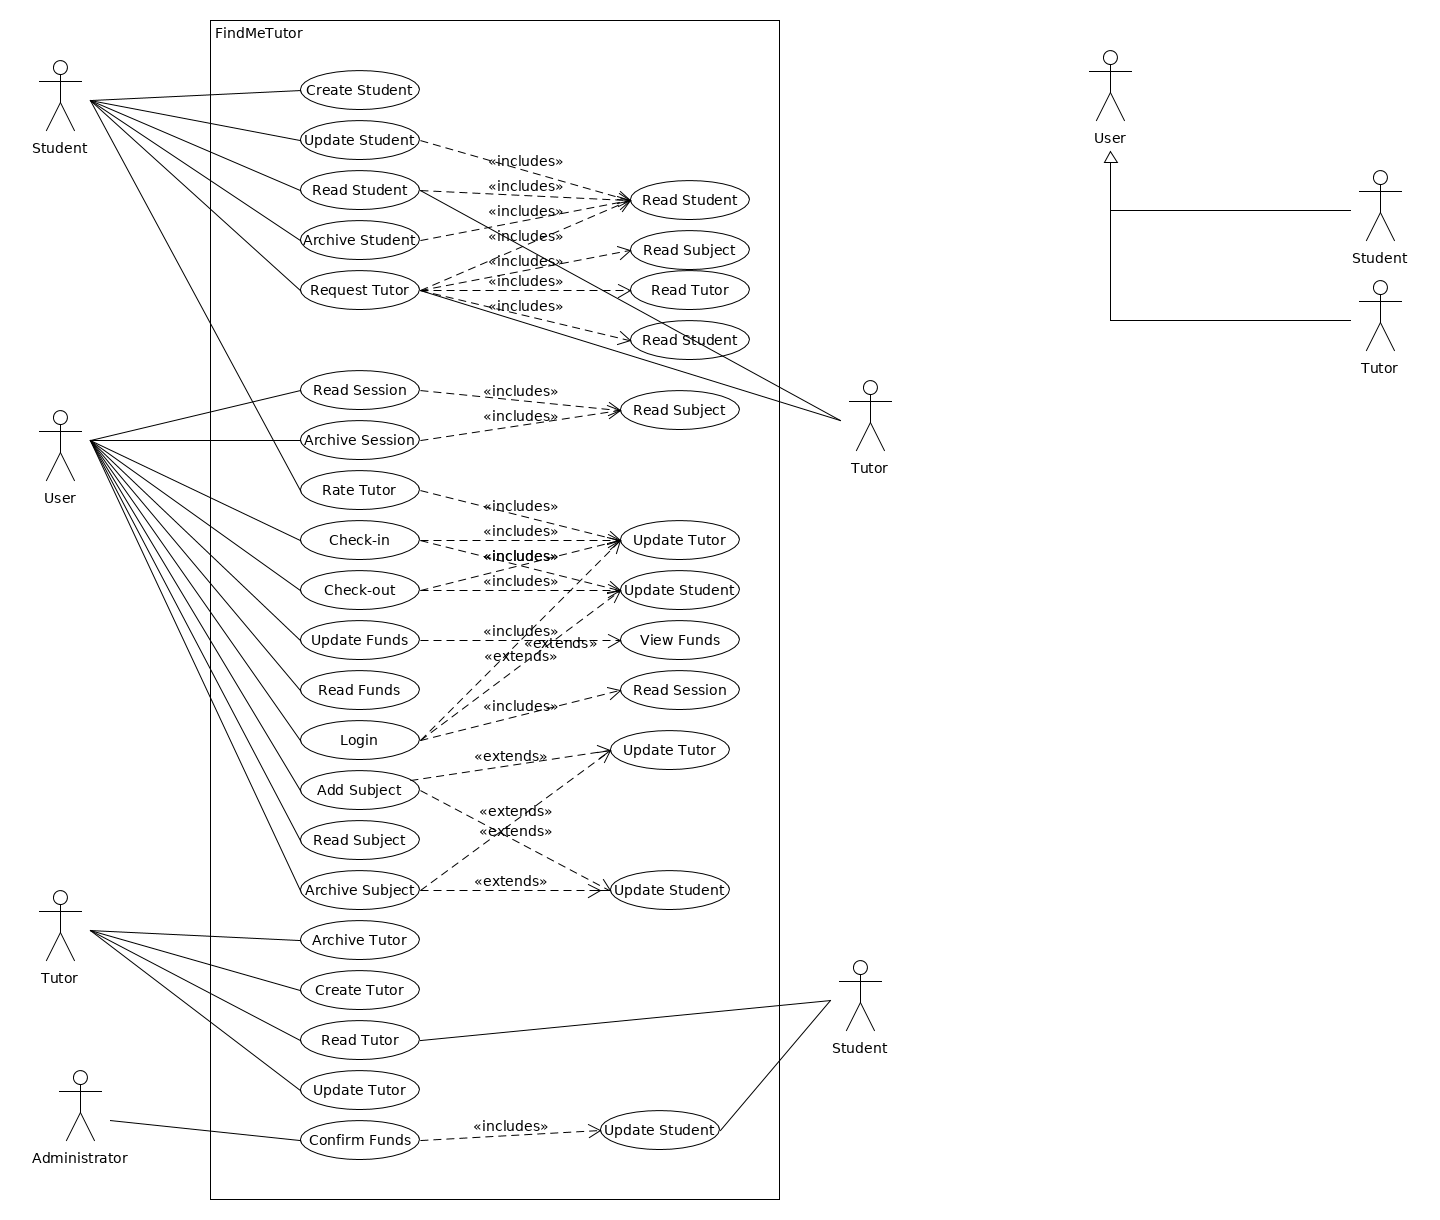
\includegraphics[width=140mm]{./Sprint3Models/Use_Case_Diagram.png}


\newpage
\subsubsection{User stories}
{

\begin{longtable}{| l | p{10cm}| l |}
			\hline
			\textbf{Identifier} & \textbf{User story} & \textbf{Size (points)}

						\\ \hline ST-1 & As a student, I want to be able to register on the FindMeTutor application so that I can log in to the application  & 5
			\\ \hline ST-2 & As a student, I want to  log in to my account on the FindMeTutor application so that I have access to the facilities on the application.  & 3
			\\ \hline ST-3 & As a tutor, I want to be able to register on the FindMeTutor application so that I can log in to the application  & 3
																\\ \hline ST-4 & As a tutor, I want to  log in to my account on the FindMeTutor application so that I have access to the facilities on the application.  & 3
																\\ \hline ST-6 & As an administrator, I want to be able to register on the FindMeTutor application so that I can log in to the application  & 3
													\\ \hline ST-7 & As an administrator, I want to  log in to my account on the FindMeTutor application so that I have access to the facilities on the application  &3

			\\ \hline ST-8 & As a student I want to be able to request a tutor so that I can request assistance.& 5
			\\ \hline ST-9 & As a student I want to add an event to my 'Upcoming events' so I can note scheduled tutorial sessions. &3

			\\ \hline ST-10 & As a student I want to amend an event on my 'Upcoming events' so that my scheduled tutorial sessions are true reflections. & 2

			\\ \hline ST-11 & As a student, I want to delete an event on my 'Upcoming events' so that my scheduled tutorial sessions are true reflections. & 2

			\\ \hline ST-12 & As a student, I want to  view an event on my 'Upcoming events' to stay informed of scheduled tutorials I have requested. & 4

			\\ \hline ST-13 & As a tutor I want to accept a tutor request so that I can inform the student that I am willing to conduct a tutorial session. &5

						\\ \hline ST-14 & As a tutor I want to  reject a tutor request so that I can inform the student that I wont be able to assist.   & 5

			\\ \hline ST-14 & As a tutor, I can  add an event to my 'Upcoming events' so I can note scheduled tutorial sessions.  & 3

			\\ \hline ST-15 & As a tutor, I can  amend an event on my 'Upcoming events' so I can note scheduled tutorial sessions.  & 2

			\\ \hline ST-16 & As a tutor, I can  delete an event on my 'Upcoming events' so I can note scheduled tutorial sessions which are of true reflection. & 2

			\\ \hline ST-17 & As a tutor, I can  view an event on my 'Upcoming events'   so I can note scheduled tutorial sessions. & 4

			\\ \hline ST-18 & As a student I want to select a tutor from the pool of tutors who have accepted the tutorial request, so that I can choose a tutor which I feel is most suitable (according to the rating obtained and their qualifications)  &5

			\\ \hline ST-19 & As a student I want to make contact with a confirmed tutor so that I can make tutorial arrangements (venue confirmation) &5

			\\ \hline ST-20 &As a tutor I want to make contact with a confirmed student so that we can make tutorial arrangements (venue confirmation)  &5

			\\ \hline ST-21 & As a student I want to check-in to a tutorial session so that my location is known to the administrator as a measure of safety.  &5

			\\ \hline ST-22 & As a student I want to check-out to a tutorial session so that my leaving of the tutorial location is known to the administrator as a measure of safety.   &5

			\\ \hline ST-23 & As a tutor I want to check-in to a tutorial session so that my location is known to the administrator as a measure of safety  &5

			\\ \hline ST-24 & As a tutor I want to check-out to a tutorial session so that my leaving of the tutorial location is known to the administrator as a measure of safety  &5


			\\ \hline ST-25 & As a student I want edit my profile so that my details are constantly up-to-date.  	 &3


			\\ \hline ST-26 & As a tutor I want edit my profile so that my details are constantly up-to-date.  &3

			\\ \hline ST-27 & As a student I want to use the 'About' function to assist in my understanding of how the app works.  &2

			\\ \hline ST-28 & As a tutor I want to use the 'About' function to assist in my understanding of how the app works.   &2

			\\ \hline ST-29 & As a student I want to rate a tutor that has tutored me, to give feedback to fellow students and to the tutor about my understanding after the tutorial session. &4

			\\ \hline ST-30 & As a student I want a payment to be made, once I have checked out, as well as once the tutor has checked out so that the payment can only be made from my account once we have both checked out as a measure of safety.  &4 \\ \hline
\end{longtable}
}


\subsubsection{Analysis object model}
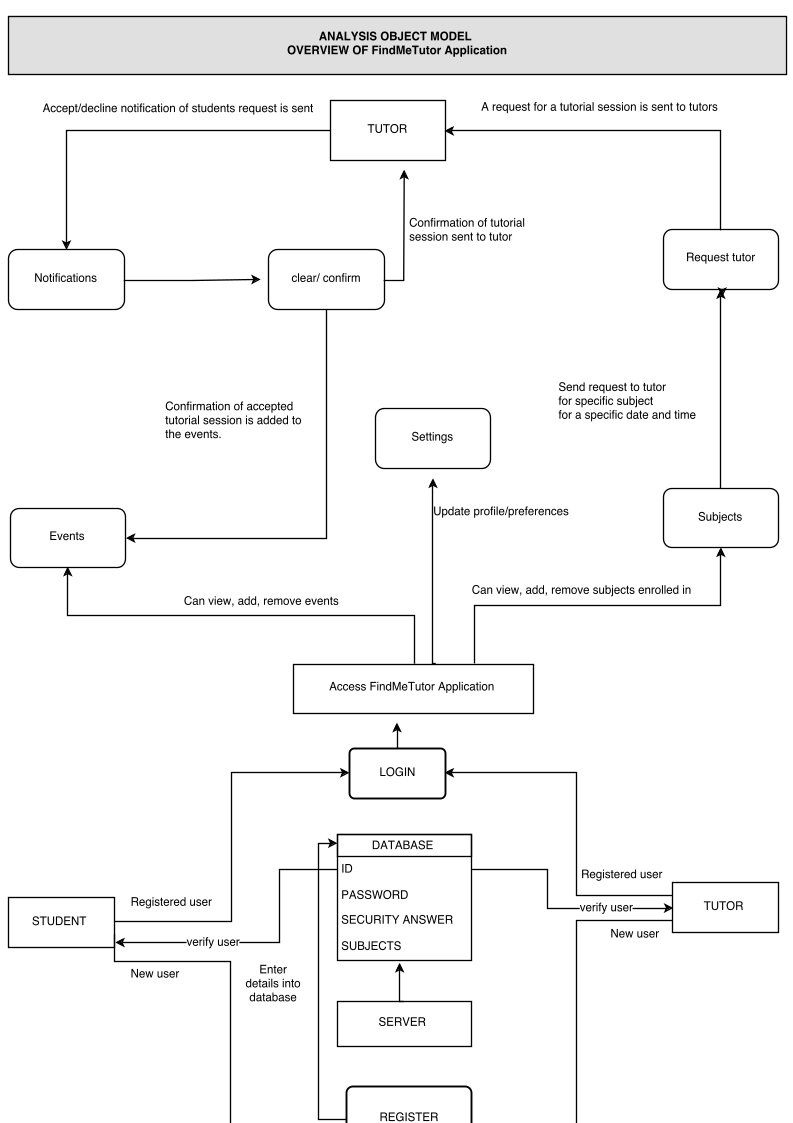
\includegraphics[width=140mm]{./Sprint3Models/Analysis_Object_model3.png}



\subsubsection{Dynamic model}
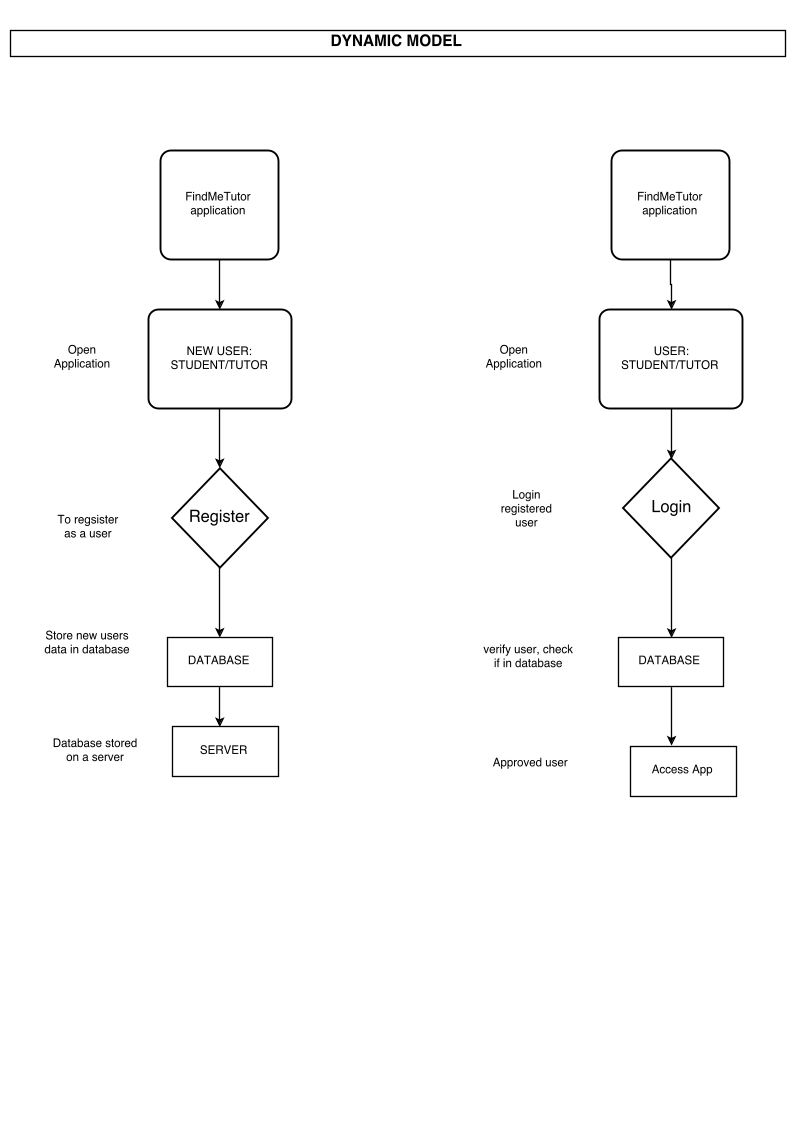
\includegraphics[width=140mm]{./Sprint3Models/Dynamic_model3.png}

%(Attached P18)
%A dynamic model represents the behaviour of an object over time. It is used where the object's behaviour is best described as a set of states that occur in a defined sequence. The components of the dynamic model are:\\
 %	States. The purchase order (PO) is modelled as passing through a set of states. The operations that can be performed on the PO are dependent on the state it is in. For example, information cannot be entered after it has reached the approved state.\\
	%State transitions. When purchase order data entry has been completed it transitions from the entering PO state to the pending approval state. State transitions are modelled as being instantaneous.\\
%	Events. Events trigger state transitions. For example, the order mailed event triggers a state transition from the approved to the placed state.\\
%	Actions. Actions occur on state transitions. For example, on a goods received event the action of notify purchaser is performed. Actions are modelled as instantaneous occurrences (contrast with activities).\\
%	Activities. An activity is performed while an object is in a specific state. For example, while in the entering PO state data is entered into the PO. Activities are modelled as occurring over a period of time (contrast with actions).\\


 \subsubsection{User interface navigational paths and screen mock-ups}
 Appendix 3

%(Attached P19)

\subsubsection{Operational requirements}

Operational requirements describe the non-business characteristics of an application.\\
\begin{flushleft}
3.5.1 Amazon Web Server - Web server to host the database
\end{flushleft}
\begin{flushleft}
3.5.2 Android studio to design UI
\end{flushleft}
\begin{flushleft}
3.5.3 GitHub to facilitate the build of the project among team members
\end{flushleft}
\begin{flushleft}
3.5.4 MySql which is the database management system used to house and control the database.
\end{flushleft}
\begin{flushleft}
3.5.5 phpMyAdmin which is used to interact with the database in a graphical user interface.
\end{flushleft}
\begin{flushleft}
3.5.6 000webhost -Web server to host the database (as Amazon web services could no longer host our application)
\end{flushleft}
\begin{flushleft}
3.5.7 Android studio: unit tests and Instrumental tests  - to run the application's unit tests
\end{flushleft}


\newpage
\section{REFERENCES}
\begin{itemize}
\item \texttt{requirements\_analysis\_document}.pdf - given in class
\item Marsic, Ivan. Software Engineering. New Jersey: Rutgers, 2012. Print.
\end{itemize}
\newpage
\section{APPENDIX}

%GLOSSARY
%\section{GLOSSARY}



\end{document}

\grid
